\section{Przypadki użycia}\label{przygotowania:przypadki-uzycia}
Uniwersalne przypadki użycia, które będą dostępne dla każdego użytkownika:
\begin{figure}[H]
    \centering
    \clearpage
    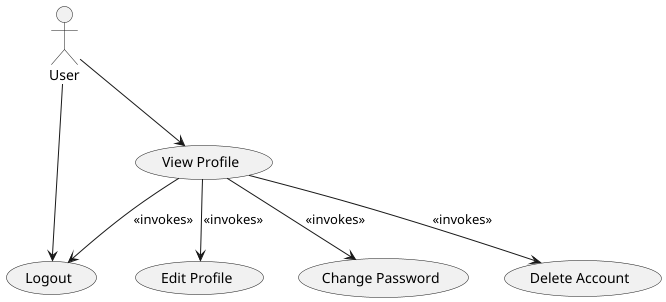
\includegraphics[width=15cm,keepaspectratio]{rysunki/usecases/UserUseCases.png}
    \caption{Przypadki użycia dla każdego użytkownika}
    \label{fig:usecases:user}
\end{figure}

Przypadki użycia, które będą dostępne dla użytkownika będącego nauczycielem:
\begin{figure}[H]
    \centering
    \clearpage
    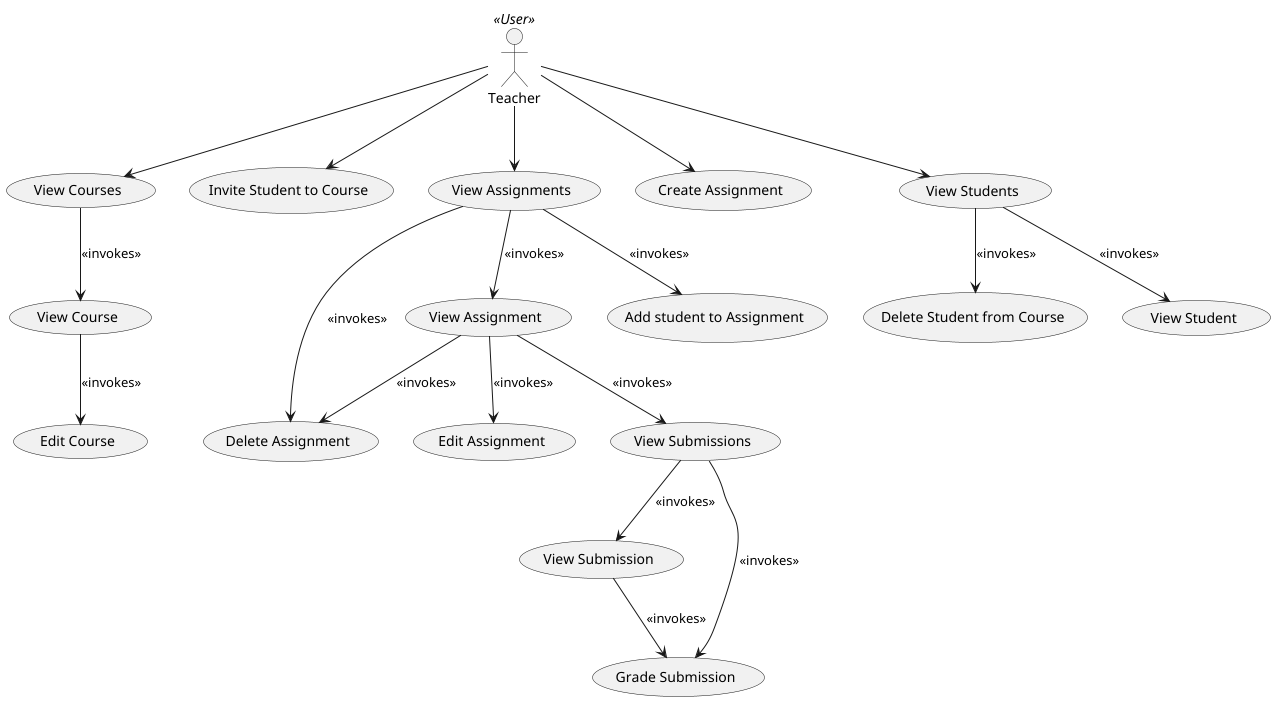
\includegraphics[width=15cm,keepaspectratio]{rysunki/usecases/TeacherUseCases.png}
    \caption{Przypadki użycia dla nauczyciela}
    \label{fig:usecases:teacher}
\end{figure}

Przypadki użycia, które będą dostępne dla użytkownika będącego uczniem:
\begin{figure}[H]
    \centering
    \clearpage
    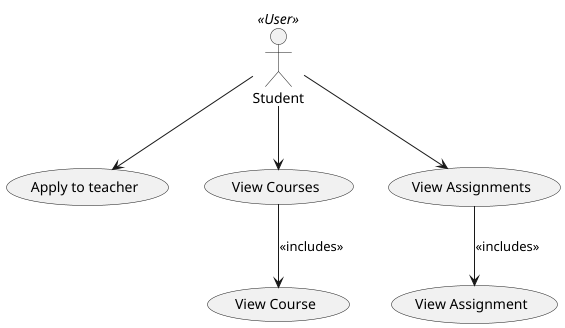
\includegraphics[width=15cm,keepaspectratio]{rysunki/usecases/StudentUseCases.png}
    \caption{Przypadki użycia dla ucznia}
    \label{fig:usecases:student}
\end{figure}

Dzięki wstępnej analizie przypadków użycia, można zauważyć, że aplikacja będzie miała kilka cech, które będą wyraźnie kształtować jej strukturę:
\begin{itemize}
    \item Będą występować role użytkowników, które będą miały dostęp do różnych funkcji aplikacji - nauczyciel, uczeń.
    \item Można wyróżnić kilka podstawowych domen funkcjonalności aplikacji:
    \begin{itemize}
        \item Uczeń
        \item Nauczyciel
        \item Autoryzacja
        \item Zadania (ang. Assignments)
    \end{itemize}
\end{itemize}

Znacząco to ułatwia rozplanowanie implementacji rozwiązania.
Autoryzacja dostępu na podstawie ról klientów serwera będzie kluczowym elementem aplikacji.
\clearpage


